\section{Probabilistic Model for Grounding Unknown Symbols} \label{sec:technical}
%In the previous section, it has been stated that the DCG model can be efficiently used in grounding problems where the objects and phrases are known and the phrases are grounded to only perceived objects. In this paper, the proposed model DCG-UPUP-Away enables the solution of a more generalized grounding problem such that 1) the phrases and objects may be known or unknown, and 2) the phrases may be grounded to objects that are out of perception. To this end, the following sections detail how to ground unknown phrases or objects, how to incrementally learn new objects and phrases, how to hypothesize groundings out of perception, and how to involve adjective attributes into grounding to avoid ambiguities.   

In this section, we extend the DCG model to infer unknown concepts. This is mainly achieved by introducing new symbols to the model. In the subsequent sections, we describe how to infer the grounding 1) unknown phrases or objects, and 2) hypothetical objects that are outside the robot's field of view. %Then, we present a method to resolve ambiguities via linguistic context, which helps to improve the grounding performance of the proposed model.

\begin{figure*}
\centering
%\begin{subfigure}[t]{0.235\textwidth}
%\centering
%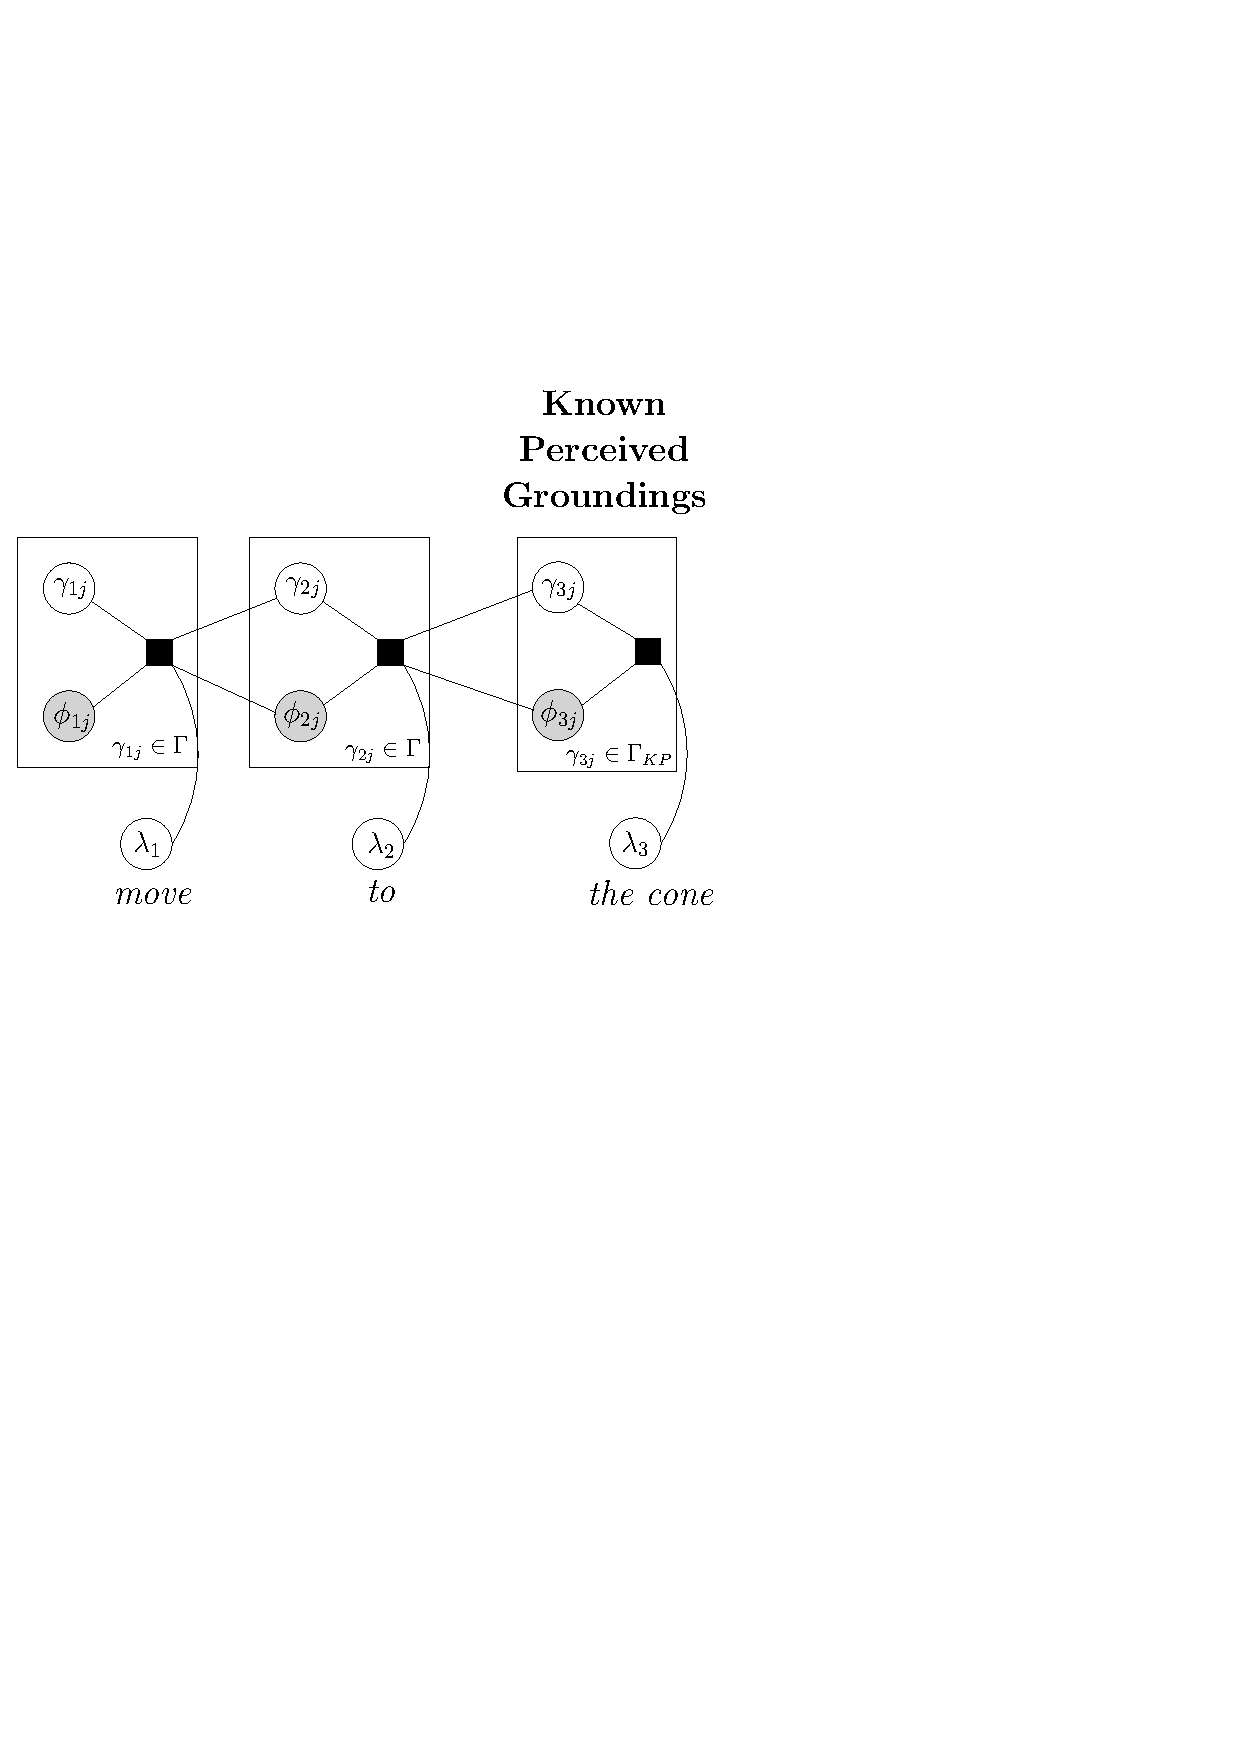
\includegraphics[width=\textwidth]{dcg.pdf}
%\caption{The DCG model}
%\label{fig:dcg}
%\end{subfigure}
%~
\begin{subfigure}[t]{0.40\textwidth}
\centering
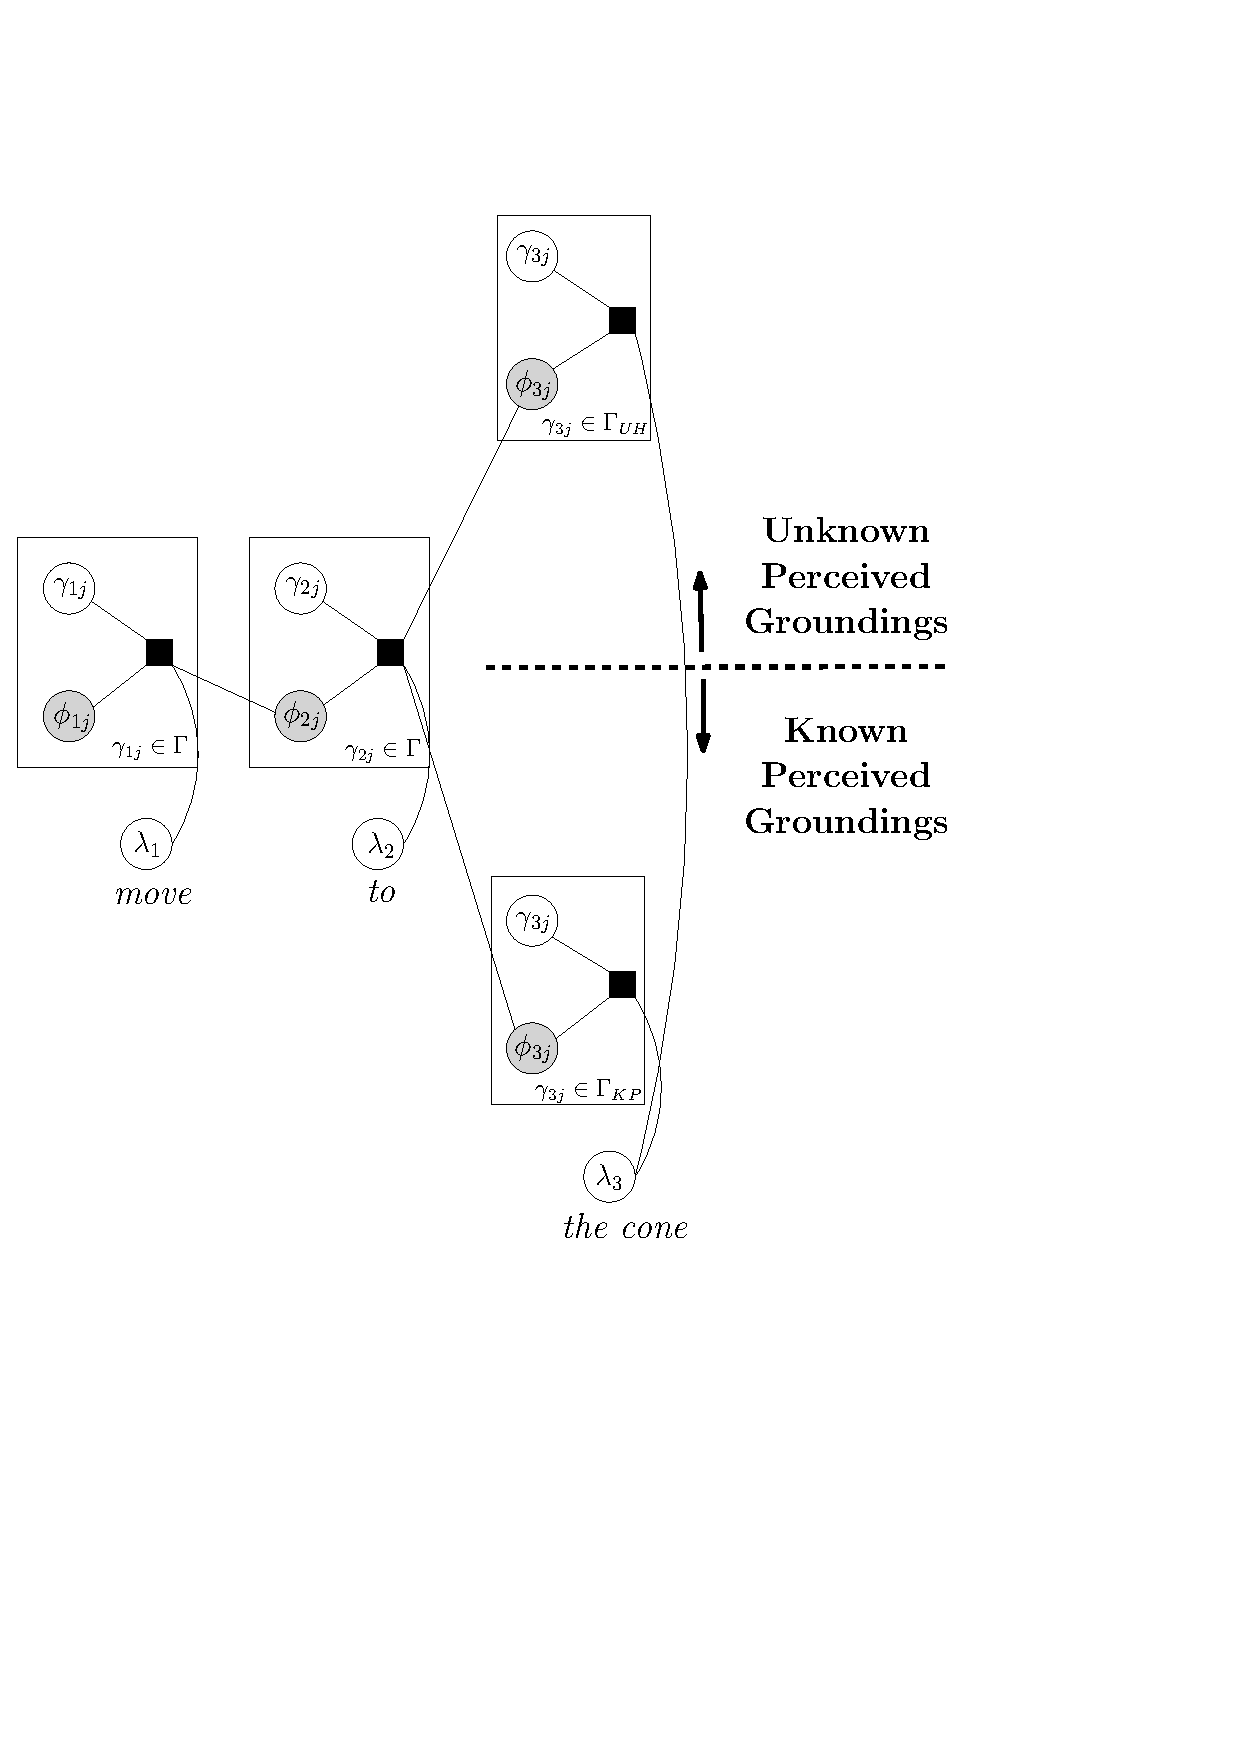
\includegraphics[width=\textwidth]{dcg_upup.pdf}
\caption{The DCG-UPUP model}
\label{fig:dcg-upup}
\end{subfigure}
~~~~
\begin{subfigure}[t]{0.52\textwidth}
\centering
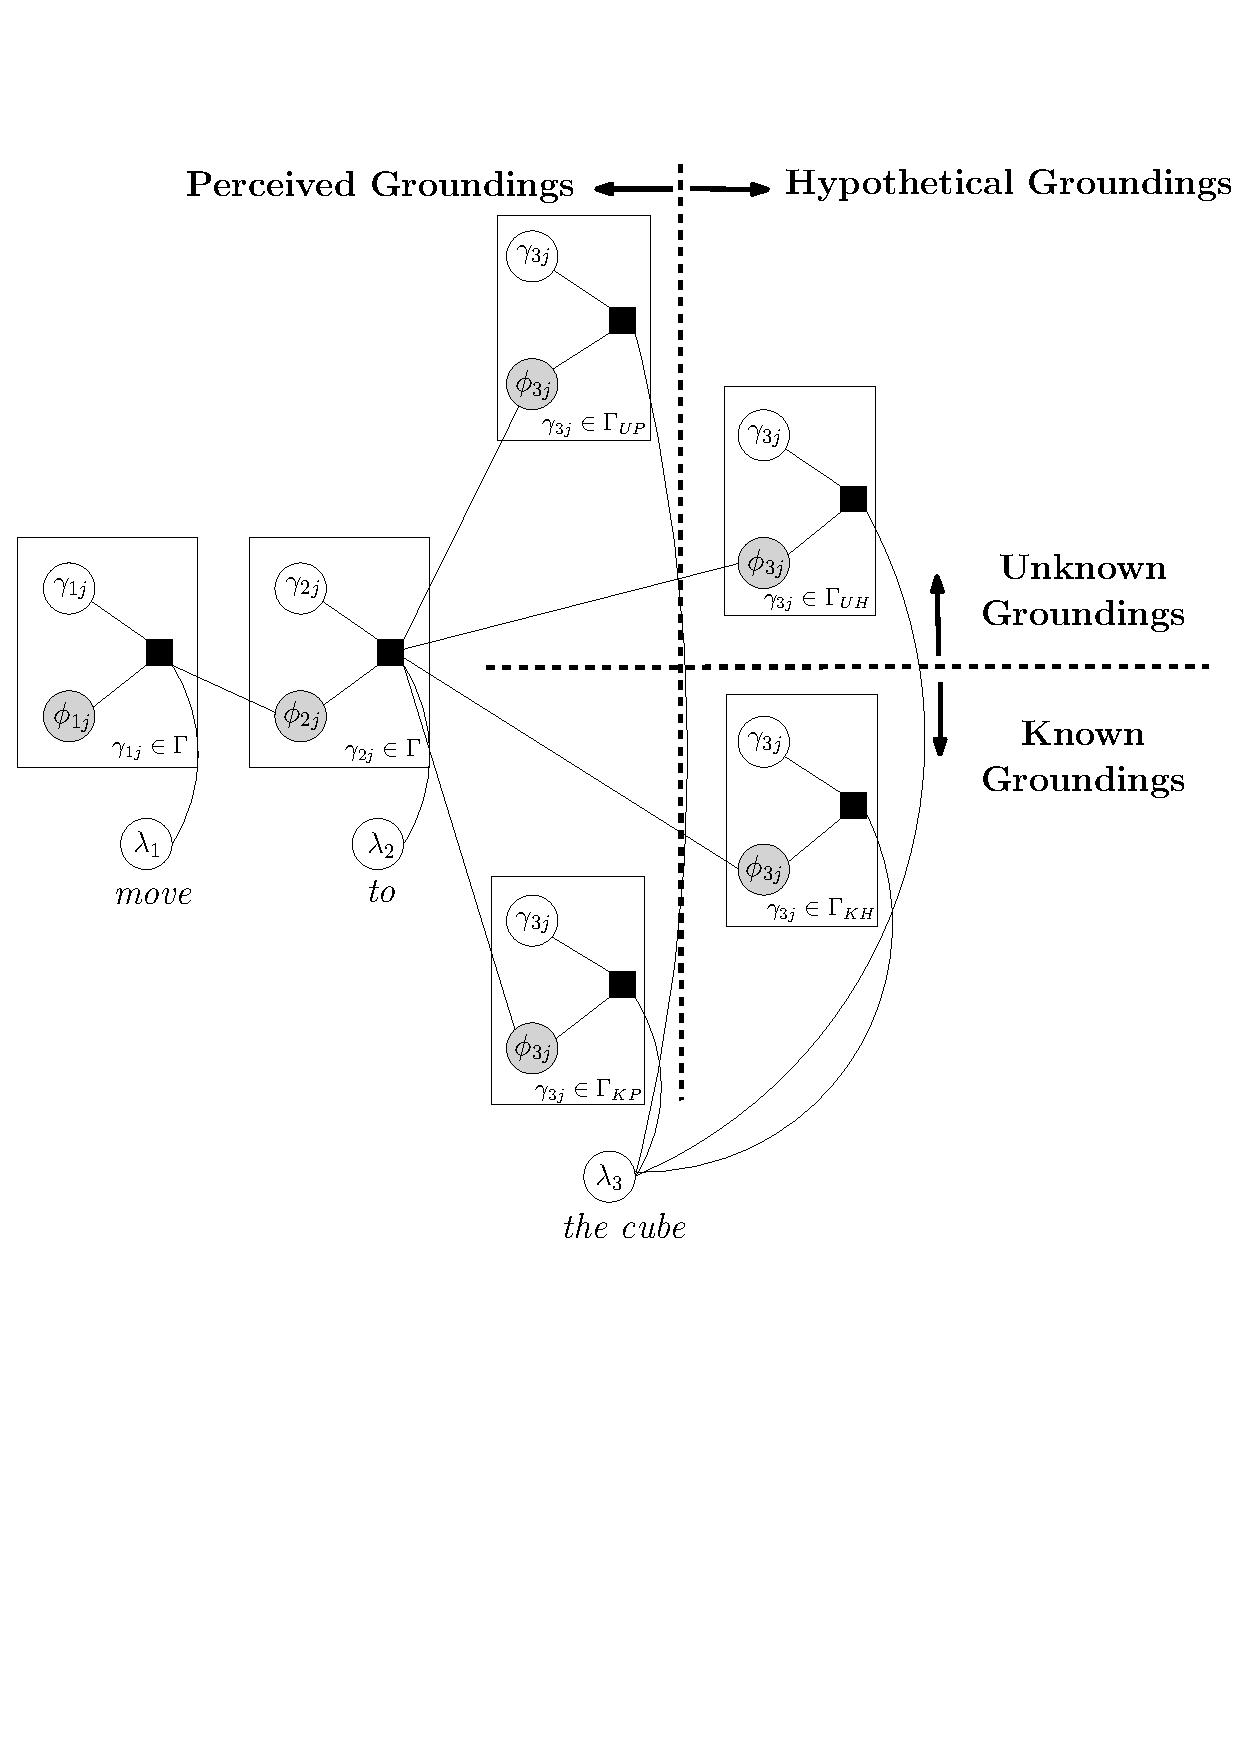
\includegraphics[width=\textwidth]{dcg_upup_away.pdf}
\caption{The DCG-UPUP-Away model}
\label{fig:dcg-upup-away}
\end{subfigure}
\caption{The graphical models instantiated for the command ``{move to the cube}". (a) The unknown groundings are explicitly represented and the grounding variables are assumed to be perceived. (b) The unknown perceived, known perceived, known hypothetical, and unknown hypothetical groundings are explicitly represented (separated by dashed lines).}
\end{figure*}

\subsection{Grounding Unknown Phrases or Objects}
%In this paper, the phrases (i.e., nouns) are
%defined as unknown if they have never grounded to a known
%object type in the training files. By maintaining a set of known
%nouns, one can easily determine whether or not a
%phrase is unknown. Similarly, the objects are defined as unknown
%if no object of the same class has ever appeared in the training
%data. 

%n this context, an object or a phrase is defined as unknown, if they have never appeared in the training. 

%An alternative model can be generated by decoupling the unknown symbols from the known symbols as in Fig.~\ref{fig:w_unknown} where each known symbol is connected to each unknown symbol (as dashed edges). While such a model represents all possible correlations between the known and unknown symbols, solving the grounding problem over this graph becomes computationally expensive due to strong connectivity.  

%Motivated by the idea of decoupling the unknown symbols from the known ones, we propose the DCG-UPUP model which exhibits a less connected graph than the one in Fig.~\ref{fig:w_unknown} (by removing the dashed edges). This simpler representation is mainly based on the following assumption: given the language command $\boldsymbol{\lambda}$ and the world model $\Upsilon$, the unknown groundings become conditionally independent from the known groundings because the variables $\boldsymbol\lambda$ and $\Upsilon$ are sufficient to predict the unknown groundings. 

In this work, a phrase is defined unknown if it has never been a part of a command in the training process. Similarly, an object is considered unknown, if it has never appeared in the world while training the model. The two main steps we take to enable grounding unknown phrases and objects are 1) to introduce a new grounding symbol to explicitly represent an unknown object and 2) to add new feature functions to identify whether an object or a phrase is unknown. Hence, the set of overall groundings can be defined as the union of unknown and known perceived groundings (i.e., $\Gamma = \Gamma_{UP} \cup \Gamma_{KP}$ \footnote{In the DCG model, $\Gamma = \Gamma_{KP}$.}), and the world model can be represented based on the known and unknown perceived objects as $\Upsilon = \Upsilon_{KP} \cup \Upsilon_{UP}$. The explicit representation of the unknown symbols is illustrated in Fig.~\ref{fig:dcg-upup}.

In the DCG model, the grounding variables are assumed to be conditional independent from each other given the phrases. Similarly, we assume that the known grounding variables are conditionally independent from the unknown grounding variables given the phrases. Note that this is illustrated in Fig.~\ref{fig:dcg-upup} by the absence of edges between the unknown and known symbols. Consequently, by using the new extended sets of groundings and the world model in \eqref{eq:llm1}, the factored  objective function for the DCG-UPUP model can be written as
\begin{equation}
\boldsymbol{\phi}^* = \argmax_{\phi_{ij} \in \boldsymbol{\phi}} \prod_{i}^{|\boldsymbol\lambda|} \prod_{j}^{|\Gamma^i_{KP} \cup \Gamma^i_{UP}|} \Psi(\phi_{ij},\gamma_{ij},\lambda_i, \Phi_{c_{i}},\Upsilon_{KP} \cup \Upsilon_{UP}).
\label{eq:dcg_upup_llm1}
\end{equation}

In addition to the set of linguistic or geometric feature functions $F_{DCG}$, in this work, we introduce a new set of binary feature functions, i.e., $F_U$, which identifies the unknown phrases and objects. For example, the identification of unknown phrases are achieved by keeping a list of known words, and then the corresponding feature $f$ checks whether a phrase in the command is in that list. On the other hand, the detection of unknown objects are realized by quantifying the classification likelihood (e.g., natural entropy \cite{grimmett2013}) of perceived objects based on the known object (image) classifiers. Accordingly, the factor function $\Psi(.)$ in \eqref{eq:dcg_upup_llm1} becomes a log-linear model with the new feature sets as follows: %by plugging the new extended sets of groundings and the features to \eqref{eq:llm1}, the factored objective function for the DCG-UPUP model can be written as      
%Motivated by the idea of decoupling the unknown symbols from the known ones, we propose an extension of the DCG model, that is the DCG-UPUP model, as illustrated in Fig.~\ref{fig:dcg-upup}. In light of going from \eqref{eq:dcg_factored1} to \eqref{eq:llm1}, the factored objective function for the DCG-UPUP model can be written as %in \eqref{eq:dcg_upup_llm1} where the the domain of the world model is extended to known and unknown perceived objects (i.e., $\Upsilon_{KP} \cup \Upsilon_{UP}$).
%where 
\begin{equation}
\Psi(.) = \frac{\exp \Big( \sum\limits_{f \in F_{\text{DCG}} \cup F_U} \mu_f f(\phi_{ij},\gamma_{ij},\lambda_i,\Phi_{c_{i}},\Upsilon_{KP} \cup \Upsilon_{UP}) \Big)}{\sum\limits_{\phi_{ij} \in \{0,1\}}\exp \Big( \sum\limits_{f \in F_{\text{DCG}} \cup F_U} \mu_f f(\phi_{ij},\gamma_{ij},\lambda_i,\Gamma_{c_{ij}},\Upsilon_{KP} \cup \Upsilon_{UP}) \Big)},
%\Psi(\phi_{ij},\gamma_{ij},\lambda_i,\Phi_{c_{i}},\Upsilon_{KP} \cup \Upsilon_{UP}) = \frac{\exp \Big( \sum_{f \in F_{\text{DCG}} \cup F_U} \mu_f f(\phi_{ij},\gamma_{ij},\lambda_i,\Phi_{c_{i}},\Upsilon_{KP} \cup \Upsilon_{UP}) \Big)}{\sum_{\phi_{ij} \in \{0,1\}}\exp \Big( \sum_{f \in F_{\text{DCG}} \cup F_U} \mu_f f(\phi_{ij},\gamma_{ij},\lambda_i,\Gamma_{c_{ij}},\Upsilon_{KP} \cup \Upsilon_{UP}) \Big)},
\label{eq:dcg_upup_llm2}
\end{equation}
%where
%\begin{equation}
%A_U= \exp \Big( \sum_{f \in F_{\text{DCG}} \cup F_U} \mu_f f(\phi_{ij},\gamma_{ij},\lambda_i,\Phi_{c_{i}},\Upsilon_{KP} \cup \Upsilon_{UP}) \Big) \nonumber
%%+ \sum_{f^\prime \in F_{U}} \mu_{f^\prime} f^\prime(\phi_{ij},\gamma_{ij},\lambda_i,\Phi_{c_{i}},\Upsilon_{KP} \cup \Upsilon_{UP}) \Big) \nonumber,
%\end{equation}
%
%\begin{equation}
%B_U= \sum_{\phi_{ij} \in \{0,1\}}\exp \Big( \sum_{f \in F_{\text{DCG}} \cup F_U} \mu_f f(\phi_{ij},\gamma_{ij},\lambda_i,\Gamma_{c_{ij}},\Upsilon_{KP} \cup \Upsilon_{UP}) \Big) \nonumber
%%+ \sum_{f^\prime \in F_{U}} \mu_{f^\prime} f^\prime(\phi_{ij},\gamma_{ij},\lambda_i,\Gamma_{c_{ij}},\Upsilon_{KP} \cup \Upsilon_{UP}) \Big), \nonumber
%\end{equation}
%%\exp \Big( \sum_{f \epsilon F_{\text{DCG}}} \mu_f f(\phi_{ij},\gamma_{ij},\lambda_i,\Gamma_{c_{ij}},\Upsilon_{KP} \cup \Upsilon_{UP}) \nonumber \\
%%\quad \quad \quad \quad \quad \quad \quad \quad \quad \quad \quad \quad 
%%+ \sum_{f \epsilon F_{\text{Unknown}}} \mu_f f(\phi_{ij},\gamma_{ij},\lambda_i,\Gamma_{c_{ij}},\Upsilon_{KP} \cup \Upsilon_{UP}) \Big)
%%\label{eq:dcg_upup_llm2}
%%\end{equation}
%$F_{DCG}$ and $F_{U}$ are the sets of hand-coded binary features used in the DCG model and for detecting unknown phrases or objects, respectively.
%\begin{figure}
%\centering
%\begin{subfigure}[t]{0.45\columnwidth}
%\centering
%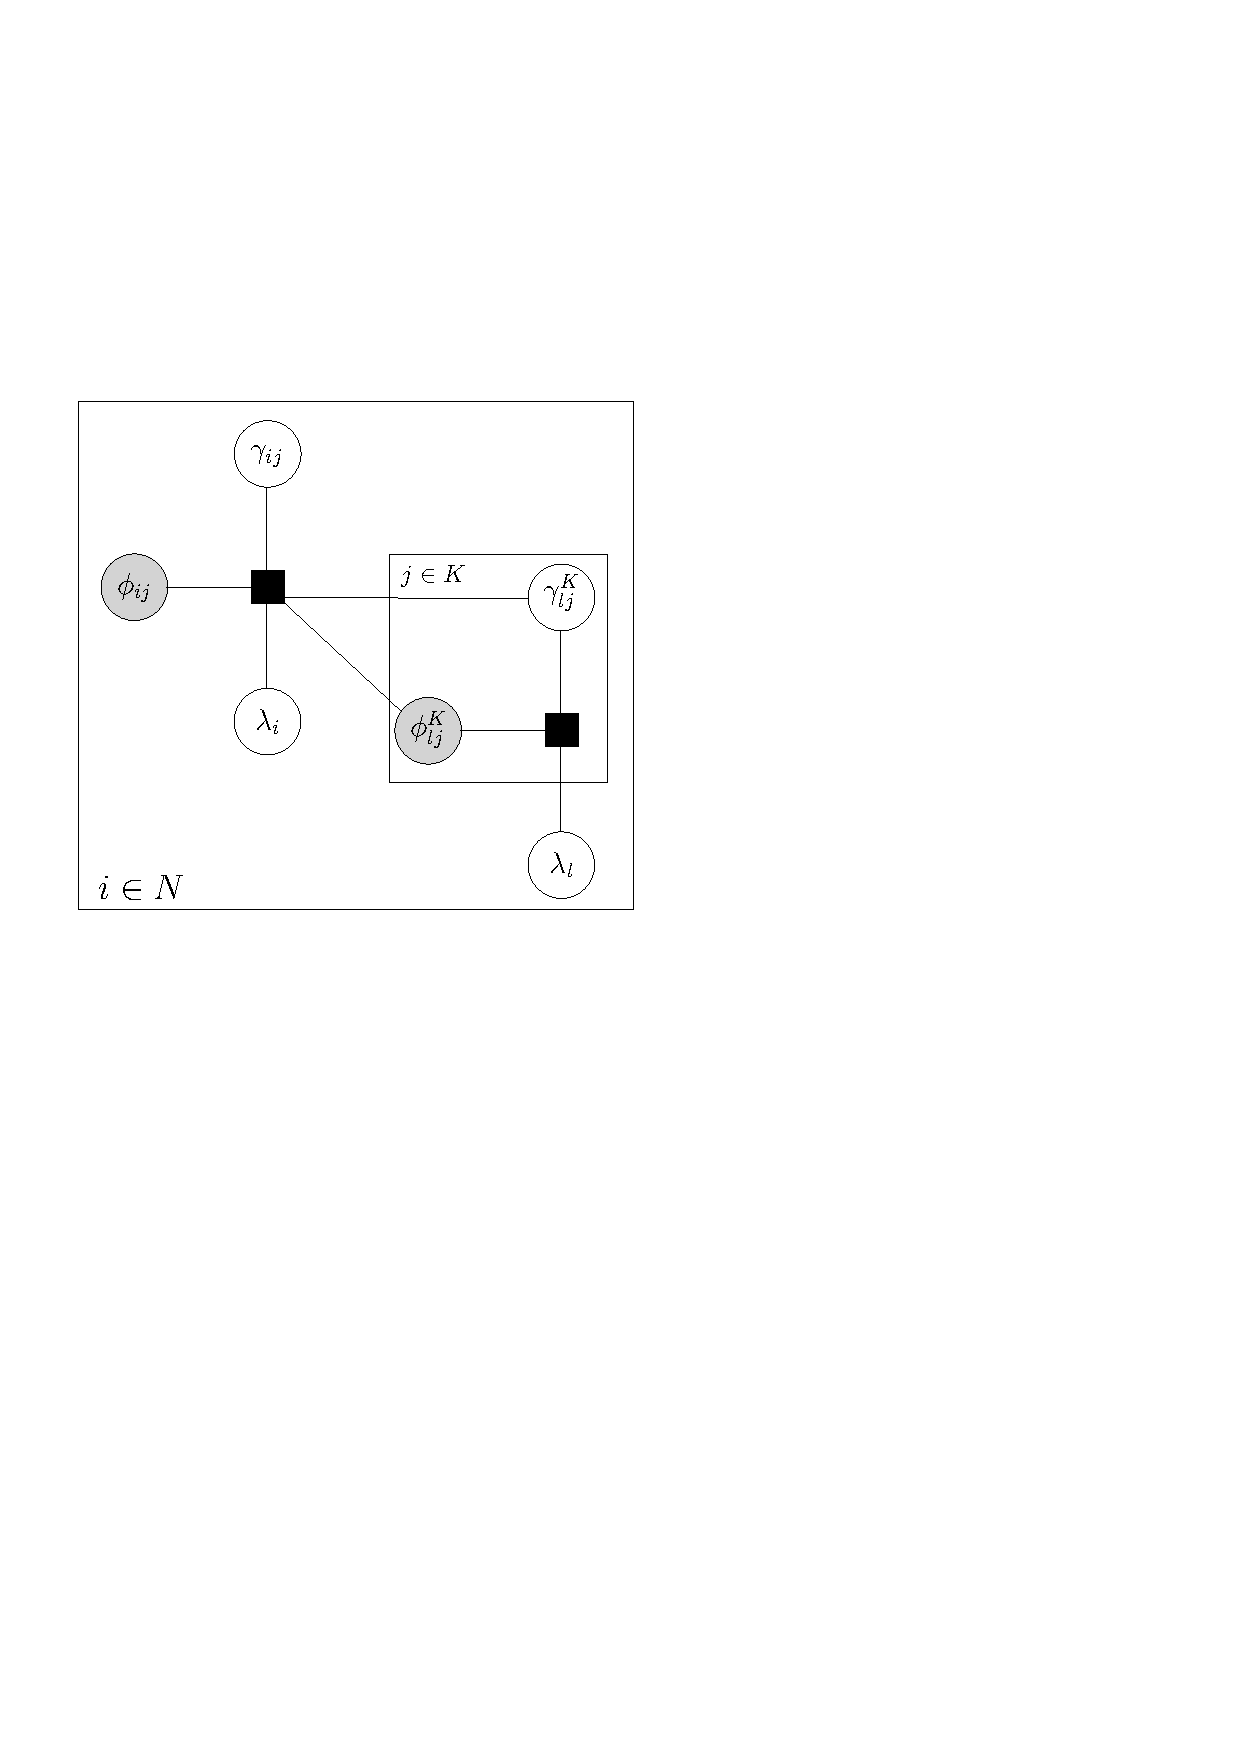
\includegraphics[width=\textwidth]{case1.pdf}
%\caption{Without explicit unknown grounding variables.}
%\label{fig:wo_unknown}
%\end{subfigure}
%~
%\begin{subfigure}[t]{0.51\columnwidth}
%\centering
%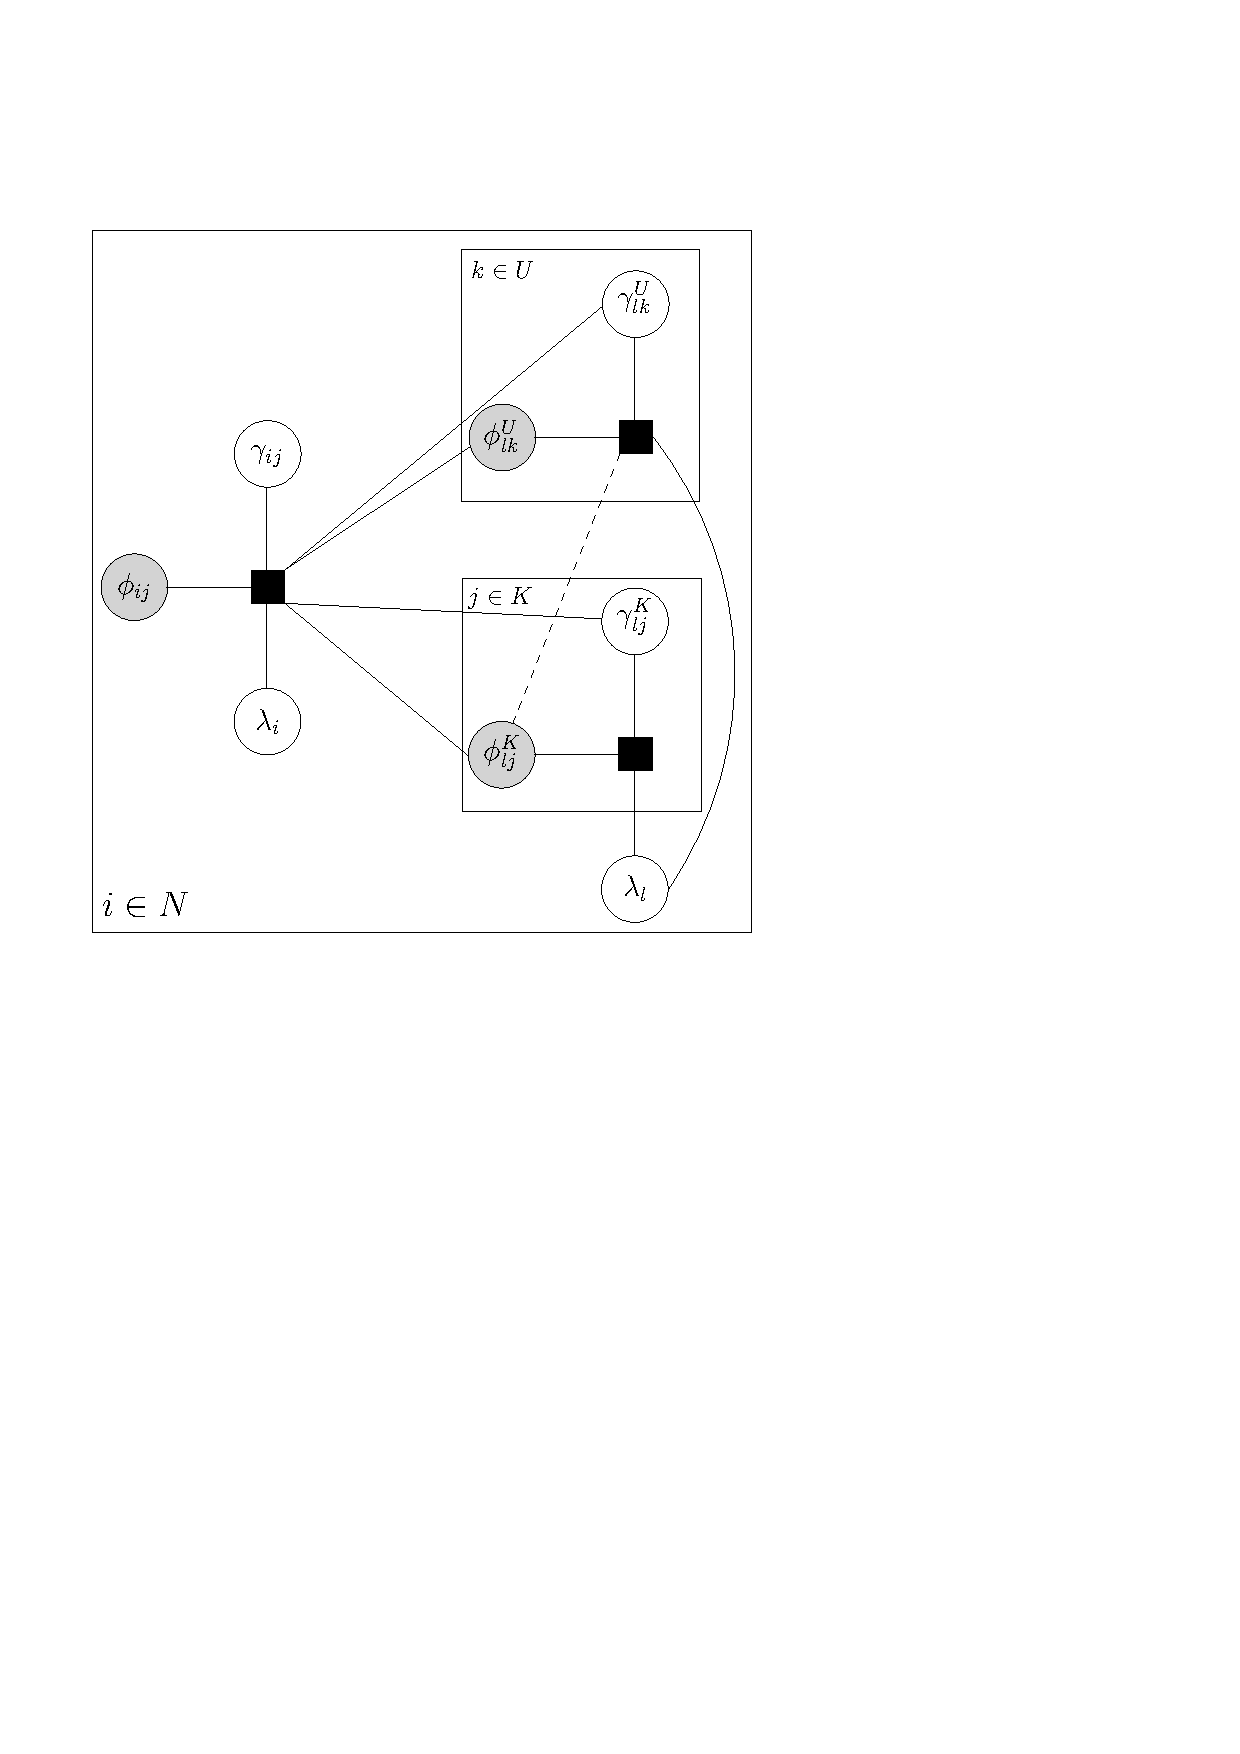
\includegraphics[width=\textwidth]{case2.pdf}
%\caption{With explicit unknown grounding variables.}
%\label{fig:w_unknown}
%\end{subfigure}
%
%\caption{Factor graph representations. Input instruction is parsed into $N$ phrases where $\lambda_l$ represents a child phrase of parent phrase $\lambda_i$. Superscripts $K$ and $U$ denote known and unknown variables, respectively.}
%\end{figure}

\subsection{Grounding Hypothetical Objects Outside the Field of View}
%The previous section presented that the DCG-UPUP model can explicitly represent the unknown phrases and objects. However, its performance is limited since the robot can only ground to the perceived objects. As an extension of this model, we introduce the DCG-UPUP-Away, which enables to ground phrases to objects that can be outside the field of view.
In this work, we define the hypothetical objects as the potential objects that can be located outside the robot's field of view. Now, we extend the DCG-UPUP model to enable grounding hypothetical objects. In existing models, the grounding is achieved based only on the objects that are perceived. However, a robot typically has a limited view of the world, and it is a strong assumption to consider that the given instructions always refer to the objects in the perceived world. To relax this assumption, we propose to add hypothetical objects to the model and let the robot associate a phrase with a hypothesized object when necessary.   

Adding hypothetical objects to the model is similar to the process of adding unknown objects to the model. First, after populating a world model by using the sensors of the robot, a single instance of every known object type, as well as one instance of an unknown object, are added to the world model and labeled as hypothetical objects. As a result, the new world model is composed of objects that are known perceived, unknown perceived, known hypothetical, and unknown hypothetical (i.e., $\Upsilon = \Upsilon_{KP} \cup \Upsilon_{UP} \cup \Upsilon_{KH} \cup \Upsilon_{UH}$). Second, new grounding symbols are added to explicitly represent the hypothetical objects. In a similar fashion, the set of groundings are extended as $\Gamma = \Gamma_{KP} \cup \Gamma_{UP} \cup \Gamma_{KH} \cup \Gamma_{UH}$. Third, a new set of binary features ($F_H$) is introduced to detect whether an object is hypothetical. For example, if the command contains an object that is not perceived based on the current field of view, then the referred object is considered hypothetical. Based on these modifications (the extensions of the world model $\Upsilon$, the grounding set $\Gamma$, and the feature functions $F$), the factored objective function for the DCG-UPUP-Away model can be written as
%As a comparison, Fig.~\ref{fig:dcg-upup} illustrates the DCG-UPUP model, where the nouns can be grounded to only known perceived and unknown perceived objects. Moreover, Fig.~\ref{fig:dcg} presents the DCG model where the nouns can be grounded to only known perceived objects.
%Similar to \eqref{eq:dcg_upup_llm1}, the factored objective function for the DCG-UPUP-Away model can be written by extending the world model to known perceived, unknown perceived, known hypothetical, and unknown hypothetical objects  (i.e., $\Upsilon_{KP} \cup \Upsilon_{UP} \cup \Upsilon_{KH} \cup \Upsilon_{UH}$) as follows:
\begin{equation}
\boldsymbol{\phi}^* = \argmax_{\phi_{ij} \in \boldsymbol{\phi}} \prod_{i}^{|\boldsymbol\lambda|} \prod_j^{|\bar\Gamma^i|} \Psi(\phi_{ij},\gamma_{ij},\lambda_i,\Phi_{c_{i}},\bar\Upsilon),
\label{eq:dcg_upup_away_llm1}
\end{equation}
where ${\bar{\Gamma}^i = \Gamma^i_{KP} \cup \Gamma^i_{UP} \cup \Gamma^i_{HP} \cup \Gamma^i_{HU}}$, $\bar\Upsilon = \Upsilon_{KP} \cup \Upsilon_{UP} \cup \Upsilon_{KH} \cup \Upsilon_{UH}$, and 
\begin{equation}
\Psi(.) = \frac{\exp \Big( \sum\limits_{f \in F_{\text{DCG}} \cup F_{U} \cup F_{H}} \mu_f f(\phi_{ij},\gamma_{ij},\lambda_i,\Gamma_{c_{ij}},\bar\Upsilon) \Big)}{\sum\limits_{\phi_{ij} \in \{0,1\}}\exp \Big( \sum\limits_{f \in F_{\text{DCG}} \cup F_{U} \cup F_{H}} \mu_f f(\phi_{ij},\gamma_{ij},\lambda_i,\Gamma_{c_{ij}},\bar\Upsilon) \Big)}.
\label{eq:dcg_upup_away_factor}
\end{equation}
%where
%\begin{equation}
%A_{UH}=\exp \Big( \sum_{f \in F_{\text{DCG}} \cup F_{U} \cup F_{H}} \mu_f f(\phi_{ij},\gamma_{ij},\lambda_i,\Gamma_{c_{ij}},\Upsilon_{KP} \cup \Upsilon_{UP} \cup \Upsilon_{KH} \cup \Upsilon_{UH}) \Big) \nonumber
%%\quad \quad \quad \quad \quad \quad + \sum_{f' \in F_{U}} \mu_{f'} f'(\phi_{ij},\gamma_{ij},\lambda_i,\Gamma_{c_{ij}},\Upsilon_{KP} \cup \Upsilon_{UP} \cup \Upsilon_{KH} \cup \Upsilon_{UH}) \nonumber \\
%%\quad \quad \quad \quad \quad \quad + \sum_{f^{\prime\prime} \in F_{H}} \mu_{f^{\prime\prime}} f^{\prime\prime}(\phi_{ij},\gamma_{ij},\lambda_i,\Gamma_{c_{ij}},\Upsilon_{KP} \cup \Upsilon_{UP} \cup \Upsilon_{KH} \cup \Upsilon_{UH}) \Big), \nonumber
%\end{equation}
%
%\begin{equation}
%B_{UH}=\sum_{\phi_{ij} \in \{0,1\}}\exp \Big( \sum_{f \in F_{\text{DCG}} \cup F_{U} \cup F_{H}} \mu_f f(\phi_{ij},\gamma_{ij},\lambda_i,\Gamma_{c_{ij}},\Upsilon_{KP} \cup \Upsilon_{UP} \cup \Upsilon_{KH} \cup \Upsilon_{UH}) \Big) \nonumber
%%\quad \quad \quad \quad \quad \quad \quad \quad + \sum_{f' \in F_{U}} \mu_{f'} f'(\phi_{ij},\gamma_{ij},\lambda_i,\Gamma_{c_{ij}},\Upsilon_{KP} \cup \Upsilon_{UP} \cup \Upsilon_{KH} \cup \Upsilon_{UH}) \nonumber \\
%%\; \quad \quad \quad \quad \quad \quad \quad \quad + \sum_{f^{\prime\prime} \in F_{H}} \mu_{f^{\prime\prime}} f^{\prime\prime}(\phi_{ij},\gamma_{ij},\lambda_i,\Gamma_{c_{ij}},\Upsilon_{KP} \cup \Upsilon_{UP} \cup \Upsilon_{KH} \cup \Upsilon_{UH}) \Big), \nonumber
%\end{equation}
%and $F_H$ is the set of hand-coded binary features to detect if an object is hypothetical. 
%\color{black}

Note that the resulting graphical model for the DCG-UPUP-Away is illustrated in Fig.~\ref{fig:dcg-upup-away}, where the nouns may ground to 1) known and perceived objects, 2) unknown and perceived objects, 3) known and hypothetical objects, and 4) unknown and hypothetical objects. 
%\subsection{Resolving Ambiguity via Linguistic Context}
%\label{sec:color}
%In real-world applications, there might exist multiple objects with the same type but different attributes. In order to resolve the ambiguities among the objects, it is crucial to allow the association between the natural language adjectives and the object properties. For example, if there exist two cube type objects in the world, one way to distinguish them from each other is to consider their properties such as color or size. In this section, we present how to include color information into the solution of grounding problem over the DCG-UPUP-Away \footnote{Other attributes such as size or shape can be included in a similar way by adding the corresponding feature functions.}. To this end, a new set of feature functions is introduced, that is $F_C = \{f_{color}, f_{word}\}$ where the feature $f_{color}$ expresses the color property of an object (e.g., whether the cube is red or not) and the feature $f_{word}$ identifies whether the language command $\boldsymbol\lambda$ contains a color adjective. Note that the addition of new features brings only a minor change to \eqref{eq:dcg_upup_away_factor} where the set of features are extended, i.e, $f \in F_{DCG} \cup F_U \cup F_H \cup F_C$. 

%One way to improve the grounding performance of the DCG-UPUP-Away model is to allow the association between the natural language adjectives and the object properties. For example, if there exist two cube type objects in the world, one way to distinguish them from each other is to consider their properties such as color or size. In this section, we present how to include color information into the solution of grounding problem over the DCG-UPUP-Away \footnote{Other attributes such as size or shape can be included in a similar way by adding the corresponding feature functions.}. To this end, a new set of feature functions is introduced, that is $F_C = \{f_{color}, f_{word}\}$ where the feature $f_{color}$ checks the color property of an object and the feature $f_{word}$ detects whether the language command $\boldsymbol\lambda$ contains a color adjective. Note that the addition of new features brings only a minor change to \eqref{eq:dcg_upup_away_factor} where the set of features are extended, i.e, $f \in F_{DCG} \cup F_U \cup F_H \cup F_C$. 

%each feature function $\Psi(.)$ is defined as follows:
%\begin{equation}
%\Psi(\phi_{ij},\gamma_{ij},\lambda_i,\Gamma_{c_{ij}},\Upsilon_{KP} \cup \Upsilon_{UP} \cup \Upsilon_{KH} \cup \Upsilon_{UH}) = \frac{A_{UHC}}{B_{UHC}}
%\label{eq:color_llm2}
%\end{equation}
%where
%\begin{equation}
%A_{UHC}=\exp \Big( \sum_{f \in F_{\text{DCG}}} \mu_f f(\phi_{ij},\gamma_{ij},\lambda_i,\Gamma_{c_{ij}},\Upsilon_{KP} \cup \Upsilon_{UP} \cup \Upsilon_{KH} \cup \Upsilon_{UH}) \nonumber \\
%\quad \quad \quad \quad \quad \quad + \sum_{f' \in F_{U}} \mu_{f'} f'(\phi_{ij},\gamma_{ij},\lambda_i,\Gamma_{c_{ij}},\Upsilon_{KP} \cup \Upsilon_{UP} \cup \Upsilon_{KH} \cup \Upsilon_{UH}) \nonumber \\
%\quad \quad \quad \quad \quad \quad + \sum_{f^{\prime\prime} \in F_{H}} \mu_{f^{\prime\prime}} f^{\prime\prime}(\phi_{ij},\gamma_{ij},\lambda_i,\Gamma_{c_{ij}},\Upsilon_{KP} \cup \Upsilon_{UP} \cup \Upsilon_{KH} \cup \Upsilon_{UH}) \nonumber \\
%\quad \quad \quad \quad \quad \quad + \sum_{f^{\prime\prime\prime} \in F_{C}} \mu_{f^{\prime\prime\prime}} f^{\prime\prime\prime}(\phi_{ij},\gamma_{ij},\lambda_i,\Gamma_{c_{ij}},\Upsilon_{KP} \cup \Upsilon_{UP} \cup \Upsilon_{KH} \cup \Upsilon_{UH}) \Big), \nonumber
%\end{equation}
%
%\begin{equation}
%B_{UHC}=\sum_{\phi_{ij} \in \{0,1\}}\exp \Big( \sum_{f \in F_{\text{DCG}}} \mu_f f(\phi_{ij},\gamma_{ij},\lambda_i,\Gamma_{c_{ij}},\Upsilon_{KP} \cup \Upsilon_{UP} \cup \Upsilon_{KH} \cup \Upsilon_{UH}) \nonumber \\
%\quad \quad \quad \quad \quad \quad \quad \quad + \sum_{f' \in F_{U}} \mu_{f'} f'(\phi_{ij},\gamma_{ij},\lambda_i,\Gamma_{c_{ij}},\Upsilon_{KP} \cup \Upsilon_{UP} \cup \Upsilon_{KH} \cup \Upsilon_{UH}) \nonumber \\
%\quad \quad \quad \quad \quad \quad \quad \quad + \sum_{f^{\prime\prime} \in F_{H}} \mu_{f^{\prime\prime}} f^{\prime\prime}(\phi_{ij},\gamma_{ij},\lambda_i,\Gamma_{c_{ij}},\Upsilon_{KP} \cup \Upsilon_{UP} \cup \Upsilon_{KH} \cup \Upsilon_{UH})\nonumber \\
%\; \quad \quad \quad \quad \quad \quad \quad \quad + \sum_{f^{\prime\prime\prime} \in F_{C}} \mu_{f^{\prime\prime\prime}} f^{\prime\prime\prime}(\phi_{ij},\gamma_{ij},\lambda_i,\Gamma_{c_{ij}},\Upsilon_{KP} \cup \Upsilon_{UP} \cup \Upsilon_{KH} \cup \Upsilon_{UH}) \Big), \nonumber
%\end{equation}
%and $F_C$ is the set of hand-coded binary features for detecting color phrases or properties (i.e., $F_C = f_{color} \cup f_{word}$).


\section{Online Learning}
\label{sec:implementation}
In this section, we propose an unsupervised online learning strategy for the model to acquire new symbols. To this end, we present an exploration phase for the robot to search for unknown objects and an incremental learning strategy to learn new symbols.
\subsection{Exploration to Find an Unknown Object}
Given a natural language command, a robot can ground the phrases within its world model by solving an inference problem over the DCG-UPUP-Away model. Consequently, a noun phrase can be grounded to a perceived (known or unknown) or a hypothetical (known or unknown) object. In the case of grounding to a hypothetical object, the robot needs to explore its surroundings to find the potential object that is referred by the phrase. There might be several exploration strategies to find the hypothetical object. In this work, we assume that the robot gradually rotates in its current position to change its field of view. As the field of view changes, the world model is updated based on the new perceived objects, and the grounding problem with the same command is solved over the DCG-UPUP-Away model until the noun phrase is grounded to a perceived object.   


\subsection{Incremental Unsupervised Learning}
Suppose that a robot is given a command with an unknown phrase. The solution over the DCG-UPUP-Away model is the association of the unknown phrase with the unknown object in the environment. When the robot perceives an unknown object as it is initially deployed, then the unknown phrase grounds to that unknown object. If the world model in its initial deployment does not contain an unknown object, it starts to explore the environment (as discussed in the previous section). Whenever it finds an unknown object, then the unknown phrase is grounded to that object. 

In addition to grounding unknown phrases to unknown objects, the model is capable of learning new symbols (objects and phrases) based on the past experience. In that case, although a robot starts a mission with a small set of known phrases and objects, it can incrementally increase its knowledge on phrases and objects and perform more efficiently in the future. To achieve this, whenever an unknown phrase is grounded to an unknown object, we propose an unsupervised learning procedure with the following steps: 
%Consequently, the unknown phrases can be grounded to unknown objects In the case of grounding to an unknown perceived object (either initially or after exploring the environment), the DCG-UPUP-Away model can reason about the corre
%While the DCG-UPUP model can reason about unknown phrases and objects, it can also learn new symbols permanently. This is mainly achieved by the following unsupervised learning procedure: whenever an unknown phrase is grounded to an unknown object, a new type is created based on the new phrase. Then, a new training example, in which the phrase grounds to the new
%type, is generated. Accordingly, the LLM models are retrained with the expanded set of training examples. Consequently, when the newly generated objects (or phrases) are encountered again, they become known symbols. Hence, the DCG-UPUP model can learn to associate a new phrase with a new type.
\vskip0.5ex
\noindent \emph{Step 1:} A new object type is created. For example, if the unknown noun phrase is "apple", a new symbolic apple-type object is created.
\vskip0.5ex
\noindent \emph{Step 2:} Based on the given command, the current world model, and the grounding solution, a new training file is created. For example, suppose that the world contains one apple, one cube, and one cone, and the robot initially knows what a cube and cone are. Let the command be ``go near the apple". Then, the DCG-UPUP-Away model will correspond to the unknown phrase ``apple" with the unknown object apple. After creating the new object type for apple as in step 1, the grounding solution is updated as corresponding the phrase ``apple" with the apple-type object. Consequently, the current world model, the given command, and the updated grounding solution constitute a new training file.
\vskip0.5ex
\noindent \emph{Step 3:} Since a new object type is created (e.g., apple-type), the set of groundings ($\Gamma$) is updated by adding the new symbolic object. 
\vskip0.5ex
\noindent \emph{Step 4:}  Since a new object type is added and an unknown phrase is grounded (from step 3), the set of features are updated as follows: first, a new feature function is created to classify whether an object corresponds to the new type. For example, several images of the apple are taken and an apple classifier is trained. Accordingly, the feature function returns true if an object is likely to be an apple based on the classifier. Second, the feature function to check whether a word is known is updated (e.g., the phrase ``apple" is added to the list of known words). 
\vskip0.5ex

Consequently, after creating a new training file and updating the set of groundings and the feature functions, the log linear model in \eqref{eq:dcg_upup_away_factor} is retrained to update the weighting functions. Hence, initially unknown symbols become known after the training.  


%\begin{algorithm}[b!]\footnotesize
%\caption{Grounding/Learning over DCG-UPUP-Away}\label{alg:dcg_upup_away}
%\begin{algorithmic}[1]
%\Procedure{DCG-UPUP-Away}{}
%\State $M \gets \text{new DCG-UPUP-Away}$
%\State $M.\Gamma \gets \text{init\_groundings}$
%\State $M.F \gets \text{init\_features}$
%\State $T \gets \text{init\_training}$
%\State $M.\text{train}(M.\Gamma, M.F, T)$
%\While {true}
%\State $\Upsilon \gets \text{perceive\_objects}(\text{camera},M.\Gamma)$
%\State $\Upsilon \gets \Upsilon + \text{hypothesize\_objects}(M.\Gamma)$
%\State $\boldsymbol{\lambda} \gets \text{get\_nl\_command}()$
%\State $[\boldsymbol{\phi}^*,\boldsymbol{\gamma}^*] \gets M.\text{ground}(\boldsymbol{\lambda},\Upsilon)$
%\If {$\boldsymbol{\gamma}^*.\text{is\_hypothesized}()$}
%\State $\text{explore\_surroundings()}$
%\Else
%\State $\text{drive\_to}(\boldsymbol{\gamma}^*)$
%\EndIf
%\State $T_u \gets \text{gen\_unsupervised\_training}(\boldsymbol{\lambda},\boldsymbol{\gamma}^*,\Upsilon)$
%\If {$\text{is\_unknown}(\boldsymbol{\lambda}) \& !\boldsymbol{\gamma}^*.\text{is\_hypothesized}()$}
%\State $\gamma' \gets \text{new\_grounding}(\boldsymbol{\lambda},\boldsymbol{\gamma}^*,\Upsilon)$
%\State $M.\Gamma \gets M.\Gamma + \gamma'$
%\State $M.F \gets M.F + f_{\text{word}}(\boldsymbol{\lambda}[\text{noun}])$
%\State $M.F \gets M.F + f_{\text{color}}(\boldsymbol{\gamma}^*[\text{color}])$
%\State $M.F \gets M.F + f_{\text{obj}}(\boldsymbol{\gamma}^*[\text{obj}])$
%\State $T_u \gets \text{replace\_unknown}(T_u,\gamma')$
%\EndIf
%\State $T \gets T + T_u$
%\State $M.\text{train}(M.\Gamma, M.F, T)$
%\EndWhile
%\EndProcedure
%\end{algorithmic}
%\end{algorithm}
%\subsection{Overview of the Pseudo-code}

%The pseudo-code for grounding and learning new symbols over the DCG-UPUP-Away model is presented in Alg.~\ref{alg:dcg_upup_away}. First, the graphical model $M$ is initialized and trained with the initial set of training data (lines 1-6). Grounding to unknown symbols and/or hypothetical objects are tackled between the lines 7-24. In particular, the world model is updated with the perceived objects (line~8) and then hypothetical objects are added (line~9). The natural language command is entered as an input (line~10). Using the model $M$ with the language command $\boldsymbol\lambda$ and the most recent world model $\Upsilon$, the grounding problem is solved (line~11). If the obtained grounding is hypothetical, then the robot initiates the exploration (line~13); otherwise the robot moves towards the grounded perceived object (line~15). Note that the exploration in this research is considered as the robot rotating in its current location. At the end of solving the grounding problem, a new training file is generated based on the given command $\boldsymbol\lambda$, the resulting grounding $\boldsymbol\gamma^*$, and the current world model $\Upsilon$ (line~16). If there exists an unknown phrase in the given command and the resulting grounding is not hypothetical, then a new object type (or grounding variable) is generated (line~18) and the set of grounding variables as well as the feature sets are updated (lines~19-22). Finally, the newly generated object type $\gamma^\prime$ replaces the unknown object type in training file $T_u$ (line~23), and the model $M$ is retrained with the new set of training data. Consequently, the initially unknown object becomes a known object in the new model $M$ in the further iterations. 



%\begin{equation}
%\Psi() = \exp \Big( \sum_{f \epsilon F_{\text{DCG}}} \mu_f f(\phi_{ij},\gamma_{ij},\lambda_i,\Gamma_{c_{ij}},\Upsilon_{KP} \cup \Upsilon_{UP} \cup \Upsilon_{KH} \cup \Upsilon_{UH}) +...\\
%\sum_{f' \epsilon F_{\text{Unknown}}} \mu_{f'} f'(\phi_{ij},\gamma_{ij},\lambda_i,\Gamma_{c_{ij}},\Upsilon_{KP} \cup \Upsilon_{UP} \cup \Upsilon_{KH} \cup \Upsilon_{UH}) +...\\
%\mu_{f_H} f_{H}(\phi_{ij},\gamma_{ij},\lambda_i,\Gamma_{c_{ij}},\Upsilon_{KP} \cup \Upsilon_{UP} \cup \Upsilon_{KH} \cup \Upsilon_{UH}) +...\\
%\sum_{f'' \epsilon F_{\text{Color}}} \mu_{f''} f''(\phi_{ij},\gamma_{ij},\lambda_i,\Gamma_{c_{ij}},\Upsilon_{KP} \cup \Upsilon_{UP} \cup \Upsilon_{KH} \cup \Upsilon_{UH}) \Big)
%\label{eq:color_llm2}.
%\end{equation}
